\section{Introduction}

% after adding detector overview, might become 4 pages

\subsection{Neutrinos as Fundamental Standard Model Particles}
The Standard Model includes three charged leptons, three neutrinos and six quarks and their antiparticles which are splitted into three generations and can interact through gauge bosons (see \ref{fig:StandardModel}). The neutrinos. neutrinos are fundamental particles of the Standard Model.\ref{ref_PDG}\\
Figure with Standard Model particles and interations. \\

\begin{figure}
\caption{Fundamental particles and interactions}
\label{fig:StandardModel}
\centering
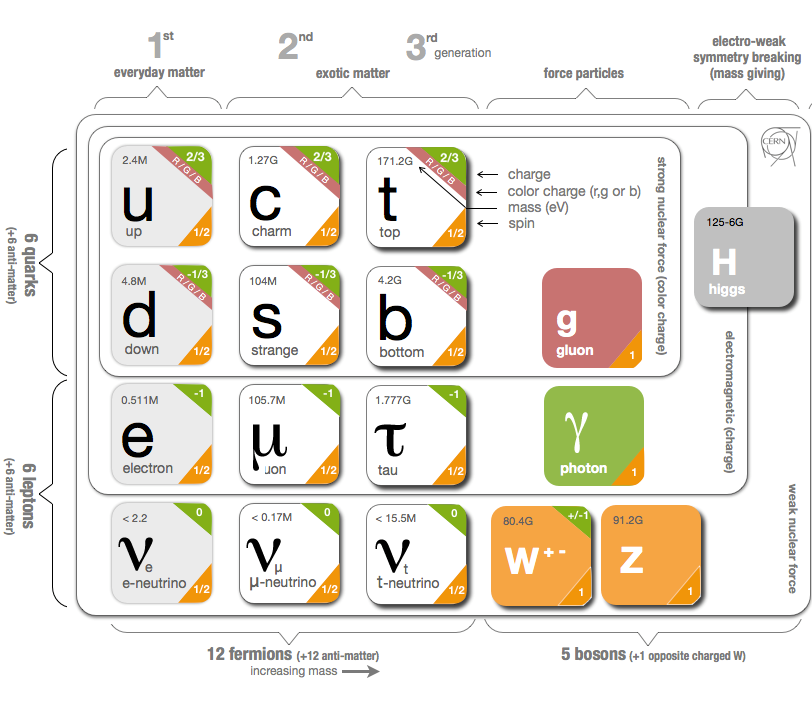
\includegraphics[width=0.8\textwidth, keepaspectratio=true]{figs/StandardModel.png}
\\Three generations of fundamental particles and interaction mediators. Charged leptons and quarks are subjects to electromagnetic interactions (through photons). Quarks can also interact strongly (through gluons). All leptons and quarks can interact weakly (through $W^{\pm}$ and $Z^0$ bosons). All the particles shown are discovered at the moment and no other fundamental particle is discovered. \cite{ref_fig_StandardModel}   
\end{figure}

How many neutrinos pass through the $cm^2$ per second (flux), check PDG.\\
Two very common and well known interactions which includes neutrinos are neutron beta decay and muon decay. The Feynmann diagrams of these processes are shown at \ref{fig:MuonAndNeutronBetaDecays}. Mean lifetime of free neutron is $~15$ minutes and $>99.9\%$ of those which decay will do it though the beta decay: $n \rightarrow p + e^- + \bar{{\nu}_e} $ \cite{ref_PDG}. At the level of fundamental particles, neutron consists of two d-quarks and one u-quark and in the beta decay one of the d-quarks transfers to u-quark though the weak interaction mediated by $W^- $ boson. Thus, the proton, which consists of two u-quark and one d-quark, is being produced. When this happens, the electron and electron antineutrino are emitted to preserve the charge and the lepton Flavor number conserved. The examples of the neutron beta decay in nature include ${^{49}}{_{19}}K \rightarrow {^{40}}{_{20}}Ca$, ${^{64}}{_{29}}Cu \rightarrow {^{64}}{_{30}}Zn$, ${^3}{_1}H \rightarrow {^3}{_2}He$ \cite{ref_Griffiths} (the positive beta decay,  $p \rightarrow n + e^+ + {\nu}_e $, is not possible for free proton but it can happen when the proton is the part of the nuclei). As for the muon, it's mean lifetime is $~2 {\mu}s$ and $~99\%$ of muons which decay would do that to electron, nuom neutrino and electron antineutrino as ${\mu}^- \rightarrow e^- + {\nu}_{\mu} + \bar{{\nu}_e}$ though the the W boson. This process is also common in nature, in cosmic rays: muon are produced in the upper layers of the Earth atmosphere from the interaction of the particles coming from cosmics with the atmosphere substances though the reaction [WHICH REACTION ?] and then some number of muons decay while traveling through the atmosphere to the ground.   

\begin{figure}
\caption{Feynmann diagrams of neutron and muon decays}
\label{fig:MuonAndNeutronDecays}
\centering
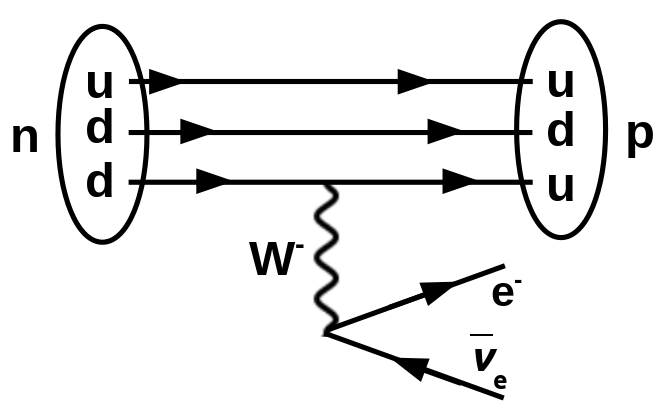
\includegraphics[width=0.3\textwidth, keepaspectratio=true]{figs/NeutronBetaDecay.png}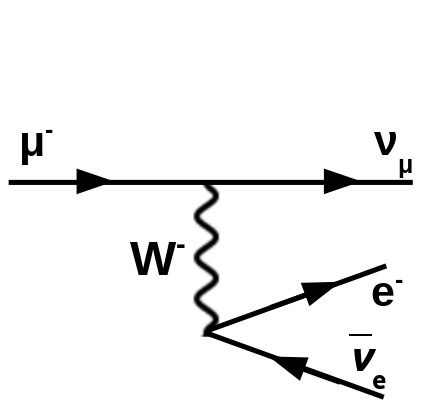
\includegraphics[width=0.3\textwidth, keepaspectratio=true]{figs/MuonDecay.png}
\\Feynmann diagrams of left: neutron beta decay \cite{ref_fig_NeutronDecay}(d-quark of transfers to u-quark through the W-boson with emission of electron and antineutrino), right:  muon decay \cite{ref_fig_MuonDecay}(muon decays to electron, neutrino and antineutrino through W-boson).
\end{figure}

There are three flavors of neutrino, one for each generation: electron neutrino, muon neutrino, tau neutrino. And in the processes described above (neutron beta decay and muon decay) the lepton flavor numbers $L_e, L_{\mu} and L_{\tau}$ are conserved. The table \ref{tab:LeptonFlavorNumber} shows the value of this number for all leptons and antileptons. 

\begin{table}[h]
  \begin{center}
  \caption{ Lepton Flavor Number}
  \begin{tabular}{|c|c|c|c|}
     particles & $L_e$ & $L_{\mu}$ & $L_{\tau}$ \\ \hline
     $e^-,\nu_e$ &  +1  &  0  &  0  \\ \hline 
     $e^+, \bar{\nu_e}$ &  -1  &  0  &  0  \\ \hline 
     $\mu^-,\nu_{\mu}$ &  0  &  +1  &  0  \\ \hline 
     $\mu^+, \bar{\nu_{\mu}}$ &  0  &  -1  &  0  \\ \hline 
     $\tau^-,\nu_{\tau}$ &  0  &  0  &  +1  \\ \hline 
     $\tau^+, \bar{\nu_{\tau}}$ &  0  &  0  &  -1  \\ \hline 
  \end{tabular}
  \label{tab:LeptonFlavorNumber}
  \end{center}
\end{table}

The lepton flavor numbers are conserved in almost all particle physics processes and the only violation of this law observed so far is the neutrino oscillations - the ability of neutrino to change flavor. This paper reviews the main idea which stands beyond the neutrion oscillations from the theoretical point of view and the related experimental measurements. Section [REFERENCE] gives theoretical derivation of the neutrino oscillations phenomenon for the two neutrinos case, introduces the mixing matrix and lists the its parameters. Section [REFERENCE] reviews the parameters which already has been measured in variety of neutrino experiments and which questions are still open. Section [REFERENCE] discusses the physical program and the technical charasteristics of the future experiment - the Long Beamline Neutrino Facility which is under construction in Fermilab now and is going to be one of the most important concentrations for the Fermilab and for the whole USA and Worldwide experimantal particle physics program in the nearest future.

\subsection{Neutrino Detection Techniques} 
Neutrinos can scatter on detector electrons throug weak neutral current (Z-boson). In this interaction, electron would leave the nuclei and would be detected. By measuring electron momentum and energy, it would be possible to receive information about original neutrino erergy and momentum but there would be no information about neutrino flavor. Also, neutrinos can interact through weak charged current ($W^\pm$-bosons) and produce charged lepton ($e^\pm$, $\mu^\pm$ or - if tau-neutrino is energetic enough - $\tau^\pm$). The properties of charged lepton can be measured in the detector and then from momentum and energy conseravation laws, the original neutrino properties will be reconstructed. Lepton flavor numbers are always conserved in these reactions and therefore it would be possible to determine the flavor of neutrino too (electron neutrino can only produce electron, muon neutrino can only produce muon and tau-neutrino can only produce tau-lepton).
The wikipedia page of Neutrino Detectors list the main detection techniques which make possible to register neutrinos \cite{ref_wiki_NeutrinoDetectors}:

\begin{figure}
\caption{Feynmann diagrams of neutrino scattering}
\label{fig:MuonAndNeutronDecays}
\centering
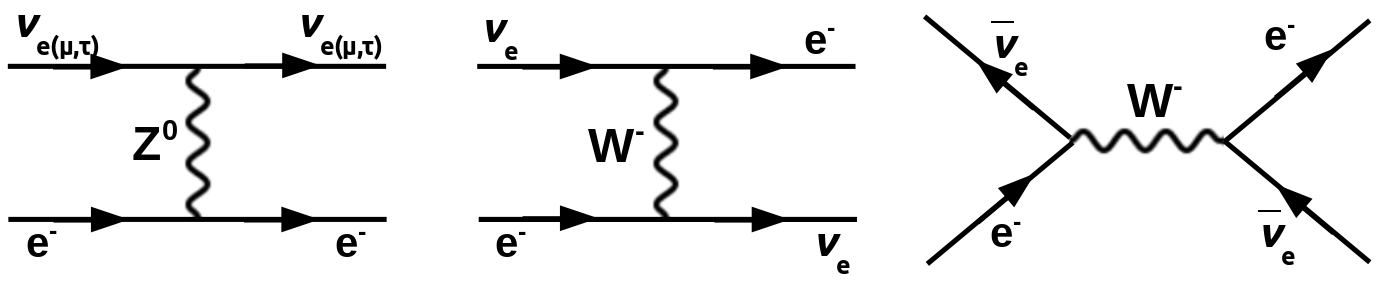
\includegraphics[width=0.9\textwidth, keepaspectratio=true]{figs/neutrinoScattering.png}
\\Feynmann diagrams of neutral current (NC, left), and neutral current (CC, middle and right) neutrino scattering.
\end{figure}
\begin{itemize}

  \item Scintillators. Was used in the first experiment which registered antineutrinos - Savannah River nuclear reactor experiment. Water with cadmium chloride solution was used as a target. Antineutrinos from the reactor interacted with protons of the target as $\bar{\nu_e}+p \rightarrow n+e^+$. Then positron annilated with electron $e^+ + e^- \rightarrow \gamma + \gamma$ and the resulting photons are detected by scintillators. The neutron is captured by the cadmium nuclei with radiation of photon. This photon is also detected by the scintillator with delay of several microseconds. 
  \item Radiochemical methods. Chlorino radiochemical detector was used in south dakota experiment: neutrino interacted with chlorine-37 atom and converted it to argon-37. Then argon atoms were separated and counted. The experiment was the first to indicate the Solar Neutrino Problem. Same idea is used in certain experiments with gallium $\rightarrow$ germanium trasformation. The radiochemical methods are only useful for counting neutrinos but can't measure their kinematic characteristics.
  \item Cherenkov detectros. A charged particle travelling through the medium with speed $v>c/n$ where $c/n$ - is speed of light in this medium radiate photons which are called Cherenkov radiation. In general, this is threshold type of detection - particle is either detected or not. However, by having several layers with different n (refractive index), it's possible to differentiate charged particles by velocities better. Common working substance for Cherenkov detectors in neutrino physics are ice, water and heavy water.
  \item Tracking calorimeters. For high energy neutrinos, neutral current weak interactions cause hadronic shower and charged current weak interactions cause electromagnetic shower. The showers produced by charged particle (product of original neutrino nteraction) identify track parameters, momentum and energy of charged particle.
\end{itemize}


\subsection{Overview of Open Questions in Neutrino Physics} 
According Particle Data Group Review \ref{ref_PDG} the following questions will be the main priority to answer by current and future neutrino experiments:
\begin{itemize}
  \item whether the massive neutrinos are Dirac or Majorana (Dirac neutrinos are... Majorana neutrinos are...)
  \item what is the sign of $\Delta{m_A}^2$ ($\Delta{m_31}^2$) and what is the type of the neutrino mass spectrum [WHAT IS THAT]
  \item what the absolute values of neutrino masses are
  \item what is the value of the neutrino mixing angle $\theta_{13}$
  \item how does the CP-symmetry behaves in the lepton sector
  \item what the values of $\Delta{m_{12}}^2$, $\theta_{12}$, and $|\Delta{m_{31}}^2|$, $\theta_{23}$.
  \item are the neutrino oscillations indication of new fundamental symmetry in particle physics
  \item what is the relation between neutrino and quark mixing if any
  \item what is the nature of the CP-violation terms in the neutrino mixing matrix
  \item can better understanding of neutrino mixing give a hint to baryon assymetry in the Universe 
\end{itemize}  

